% указываем класс документа
\documentclass[12pt,a4paper,openany]{extarticle}

% подключаем собственный стилевой файл 
\usepackage{mystyle}

% указываем язык (для автоматической вставки слов, типа "Глава", "Содержание", "Литература", "рис." и пр.
\selectlanguage{russian}

\begin{document}

\part*{Лабораторная работа №5\\
Расчет коэффициентов регулятора на примере робота~--- модели обратного маятника}

\section{Теоретические сведения}
\hspace*{\parindent}В~данной лабораторной мы закончим создание устройства, работу над которым начали в прошлый раз.
В~ней мы получим для нашего робота управляющий алгоритм, обеспечивающий его нужное поведение.

\paragraph*{Введение}$\phantom{-}$\\
\hspace*{\parindent}Опираясь на полученное в предыдущей работе уравнение движения исследуемой системы, рассмотрим наше техническое задание более подробно.
 
Учитывая физический смысл элементов матрицы $x$, несложно заключить, что, для того чтобы застабилизировать маятник в вертикальном положении, управляющему воздействию достаточно обеспечить равенство нулю двух из них~--- величин $\psi$ и $\dot\psi$. 
При этом значение третьей компоненты~--- скорости $\dot\theta$~--- может быть любым, а следовательно контролироваться не обязано.
Однако, если поддерживать его равным нулю, то, очевидно, это никак не нарушит работоспособность системы, а приведет лишь к тому, что робот помимо балансировки будет стараться остановиться в своем текущем положении.
По этой причине выберем в качестве уравнения для управляющего воздействия (напряжения, подаваемого на двигатели) следующее выражение
\begin{gather}
	U(t) = k_0(0 - \psi) + k_1(0 - \dot\theta) + k_2(0 - \dot{\psi})\label{control_form1}\\
	U(t) = -k_0\psi - k_1\dot\theta - k_2\dot{\psi}\label{control_form2},
\end{gather}  
где $k_0$, $k_1$ и $k_2$~--- некоторые постоянные.

Чтобы как-то пояснить происхождение именно такого вида функции $U(t)$, достаточно отметить, что перед нами стоит задача поддерживать значения величин $\psi$, $\dot\psi$ и $\dot\theta$ равными нулю и что подобную мы уже решили в лабораторной~№3 использованием П-регулятора.
Как там, так и здесь управляющее воздействие формируется прямо пропорциональным отклонению регулируемых переменных от их желаемых значений. 
При этом то, что в данном случае напряжение в каждый момент времени складывается из трех составлящих, не нарушает работоспособность алгоритма.

Следует заметить, что входящие в выражения для $U(t)$ постоянные коэффициенты способны иметь только определенные значения.
В~противоположность этому в лабораторной~№3 коэффициент пропорциональности мог быть практически любым: его значение сказывалось лишь на второстепенных характеристиках системы таких, как, например, быстродействие, но не нарушало её работоспособность.

Тому, как их рассчитать, главным образом, и посвящена данная лабораторная.

\paragraph*{Расчет коэффициентов для управляющего воздействия}$\phantom{-}$ \\
\hspace*{\parindent}В~прошлой работе мы получили следующее уравнение, описывающее работу исследуемой системы:
\begin{equation}\label{dx=Ax+Bu}
	\dot x = Ax + Bu\ldotp
\end{equation}
Дополнив его еще одним уравнением, справедливым для нашего робота, получим систему матричных уравнений, называемую \textit{моделью <<вход-состояние-выход>>} исследуемого объекта управления:
\begin{equation}
	\left\{
	\begin{aligned}
		\!&\dot x = Ax + Bu \\
		\!&y = Cx,
	\end{aligned}
	\right.
\end{equation}
где 
$x$~--- $n$-мерный вектор состояния системы ($n$~--- количество переменных в векторе состояния (в нашем случае $n=3$); также $n$ называют \textit{порядком объекта управления}); \\
$y$~--- $l$-мерный вектор выходных величин ($l$~--- количество переменных в нем; в нашем случае $l=3$, потому что в качестве выходных переменных мы рассматриваем все величины, входящие в $x$);\\
$u$~--- $m$-мерный вектор управляющих воздействий ($m$~--- количество переменных в нем (в нашем случае $m=1$));\\
$A$~--- матрица, определяющая динамические свойства объекта управления, размерности $n\times n$;\\
$B$~--- матрица входа управляющих воздействий размерности $n\times m$;\\
$C$~--- матрица выхода размерности $l\times n$ (в нашем случае, поскольку $x$ = $y$,
\begin{equation}
	C = 
	\begin{bmatrix}
		1 & 0 & 0\\
		0 & 1 & 0\\
		0 & 0 & 1
	\end{bmatrix} = I,
\end{equation}
где $I$~--- единичная матрица).

Прежде, чем приступить к каким-либо расчетам, необходимо проверить, а возможно ли вообще управлять нашей системой.
Для этих целей в рассмотрение вводится так называемая \textit{матрица управляемости} $Y$\!, формируемая как\footnote{Данная запись означает, что упоминаемые матрицы следует записать рядом и полученный результат рассматривать как новую матрицу.
Например,
\begin{equation*}
	O_1=
	\begin{bmatrix}
		1 & 2\\
		3 & 4
	\end{bmatrix}\!\!,\quad
	O_2=
	\begin{bmatrix}
		9\\
		8 
	\end{bmatrix}\!\!,\quad
	O_3 = [O_1\ O_2] =
	\begin{bmatrix}
		1 & 2 & 9\\
		3 & 4 & 8
	\end{bmatrix}\!\!\ldotp
\end{equation*}}
\begin{equation}
	Y = 
	\begin{bmatrix}
		B & AB & A^2B & \dots & A^{n-1}B
	\end{bmatrix}\!\!,	 
\end{equation}
и вычисляется ее определитель. 
В~случае, если $\det Y\ne0$, система управляема и синтез регулятора возможен. 
Иначе остается заключить, что наш объект неуправляем.

После удовлетворительного результата проверки введем новые матрицы $e$ и $K$, равные
\begin{gather}
	e = -x,\label{e_vector}\\
	K =
	\begin{bmatrix}
		k_0 & k_1 & k_2
	\end{bmatrix}\!\ldotp
\end{gather}

Надо сказать, что в общем случае данные матрицы строятся следующим образом.
\textit{Вектор ошибок} $e$ определяется согласно выражению
\begin{equation}
	e = x_0-x,
\end{equation}
где $x_0$~--- вектор, в котором хранятся желаемые значения всех контролируемых величин.
Поскольку в нашем случае он равен
\begin{equation}
	x_0 = 
	\begin{bmatrix}
		0\\0\\0
	\end{bmatrix}\!\!,
\end{equation}
то и получается выражение~\eqref{e_vector}.
Матрица же $K$ в общем виде выглядит как
\begin{equation}
	K =
	\begin{bmatrix}
		k_{11} & k_{12} & \cdots & k_{1n} \\
		k_{21} & k_{22} & \cdots & k_{2n} \\
		\vdots & \vdots & \ddots & \vdots \\
		k_{m1} & k_{m2} & \cdots & k_{mn}
	\end{bmatrix}\!\!,
\end{equation}
и, следовательно, имеет размерность $m\times n$.

Используя введенные матрицы, представим $u$ согласно выражению~\eqref{control_form2} в виде
\begin{equation}
	u = Ke\ldotp
\end{equation}
C~учетом новых обозначений уравнение~\eqref{dx=Ax+Bu} можно переписать как
\begin{equation}\label{model_on_e}
	\dot e = Ae-BKe = (A-BK)e = Fe\ldotp
\end{equation}
В~таком виде с ним следует работать дальше.

Поведение исследуемой системы зависит от вида \textit{характеристического полинома} матрицы~$F$:
\begin{equation}
	D(\lambda) = \det(\lambda I - F) = \lambda^n + z_{n-1}\lambda^{n-1} + z_{n-2}\lambda^{n-2} + \dots + z_{2}\lambda^{2} + z_{1}\lambda + z_0,
\end{equation}
где $\lambda$~--- <<обычная>> (никак не определяемая) переменная; $I$~--- как и ранее, единичная матрица; $z_i$ ($i\in{0,1,2,\dots,n-2, n-1}$)~--- числовые коэффициенты, получающиеся при расчете.
При этом требуемому поведению системы~--- поддержке нулевых значений компонент матрицы~$e$, определенному ее быстродействию и проч.~--- будет соответствовать определенный вид (определенные значения коэффициентов $z_i$) характеристического полинома:
\begin{equation}\label{poly_needed}
	D^*(\lambda) = \lambda^n + z^*_{n-1}\lambda^{n-1} + z^*_{n-2}\lambda^{n-2} + \dots + z^*_2\lambda^2 + z_1^*\lambda + z^*_0\ldotp
\end{equation}

Последний полином задается разработчиком в соответствии с тем, какие характеристики (какое поведение) он хочет видеть у разрабатываемой системы.
При этом (опять же в зависимости от желаемого поведения системы) применяются различные методы расчета постоянных коэффициентов $z^*_i$ ($i\in{0,1,2,\dots,n-2, n-1}$).
В~данной работе их значения следует получить раскрытием по биному Ньютона выражения
\begin{equation}\label{poly's}
	D^*(\lambda) = (\lambda+w_0)^n\!\!,
\end{equation}
где $w_0$~--- числовое значение, рассчитываемое по формуле
\begin{equation}
	w_0 = \frac{t^*_n}{t_n},
\end{equation}
где, в свою очередь,  $t_n^*$~--- <<стандартное>> значение \textit{времени переходного процесса}, определяемое по порядку объекта управления  из таблицы~\ref{tabl};  $t_n$~--- <<действительное>> значение времени переходного процесса в нашей системе.
Для первого раза последнее можно взять равным, например, $0.5$~c.
В~данной работе под этими параметрами следует понимать некоторые величины, обратно пропорциональные быстродействию робота.
То есть, например, уменьшение параметра $t_n$ при расчетах будет означать, что коэффициенты, получающиеся в результате, будут обеспечивать большее быстродействие технической системы.

\begin{table}[h!]
	\begin{equation*}
		\begin{array}{|c|c|c|c|c|c|c|}\hline
			\phantom{aa}n\phantom{aa} & \phantom{aa}1\phantom{aa} & \phantom{aa}2\phantom{aa} & \phantom{aa}3\phantom{aa} & \phantom{aa}4\phantom{aa} & \phantom{aa}5\phantom{aa} & \phantom{aa}6\phantom{aa} \\ \hline
			t_n^*,\text{ c} & 3.0 & 4.8 & 6.3 & 7.8 & 9.2 & 10.5 \\\hline
		\end{array}
	\end{equation*}
	\caption{Значения параметра $t_n^*$ в зависимости от порядка объекта управления.}
	\label{tabl}
\end{table}

Характеристический полином матрицы $F$ будет равен заданному разаботчиком, если будет справедливым соотношение
\begin{equation}\label{D(l)=D*(l)}
	D(\lambda) = D^*(\lambda),
\end{equation}
которое равносильно $n$ уравнениям вида
\begin{equation}
	z_i = z_i^*,
\end{equation}
где опять же $i\in{0,1,2,\dots,n-2, n-1}$.
В~лице данных соотношений мы получим $n$ уравнений относительно $k_0$, $k_1$, \ldots, $k_{n-1}$.
Их решением и находятся те значения элементов матрицы~$K$, которые обеспечивают истинность равенства~\eqref{D(l)=D*(l)}, а следовательно и требуемое поведение системы. 

Помимо обозначенного существуют и другие методы нахождения коэффициентов $k_0$, $k_1$, \ldots, $k_{n-1}$, которые при расчетах, производимых на ЭВМ, оказываются более удобными.
Рассмотрим их.

\paragraph*{Метод расчета коэффициентов, использующий приведение математической модели к канонической форме\footnote{В~данном методе подразумевается, что матрица $B$ имеет размерность $n\times1$.
Мы имеем дело как раз с таким случаем.}}$\phantom{-}$ \\
\hspace*{\parindent}Можно заметить, что если бы матрицы $A$ и $B$ в уравнении~\eqref{dx=Ax+Bu} были равны
\begin{equation}\label{dreams}
	A =
	\begin{bmatrix}
		0 & 1 & 0 & \ldots & 0\\
		0 & 0 & 1 & \ldots & 0\\
		\vdots & \vdots & \vdots & \ddots & \vdots\\
		0 & 0 & 0 & \ldots & 1\\
		-a_0 & -a_1 & -a_2 & \ldots & -a_{n-1}
	\end{bmatrix}\!\!,\qquad
	B  =
	\begin{bmatrix}
	0\\
	0\\
	\vdots\\
	0\\
	1
	\end{bmatrix}\!\!,
\end{equation}
где $a_i,$ $i\in\{0,1,2\ldots n-1\}$~--- некоторые числа,
то характеристический полином $\det(\lambda I - F)$ матрицы $F$ принял бы очень простую форму (пишем пример для случая $n = 3$):
\begin{equation}
	F = A - BK= 	
	\begin{bmatrix}
		0 & 1 & 0\\
		0 & 0 & 1\\
		-a_0 & -a_1 & -a_2 
	\end{bmatrix}-
	\begin{bmatrix}
		0\\
		0\\
		1
	\end{bmatrix}
	\begin{bmatrix}
		k_{0} & k_{1} & k_{2}
	\end{bmatrix}
	=
	\begin{bmatrix}
		0 & 1 & 0\\
		0 & 0 & 1\\
		-a_0-k_{0} & -a_1-k_{1} & -a_2-k_{2}
	\end{bmatrix}\!\!,
\end{equation}
\begin{equation}\notag
	D(\lambda)\!=\!
	\det\left(
	\begin{bmatrix}
		\lambda & 0 & 0\\
		0 & \lambda & 0\\
		0 & 0 & \lambda
	\end{bmatrix} - 
	\begin{bmatrix}
		0 & 1 & 0\\
		0 & 0 & 1\\
		-a_0-k_{0} & -a_1-k_{1} & -a_2-k_{2}
	\end{bmatrix}\right)
	\!=\!
	\begin{vmatrix}
		\lambda & -1 & 0\\
		0 & \lambda & -1\\
		a_0 + k_0 & a_1+k_1 & \lambda + a_2 + k_2
	\end{vmatrix}=
\end{equation}
\begin{equation}
	= \lambda
	\begin{vmatrix}
		\lambda & -1\\
		a_1+k_1 & \lambda + a_2 + k_2
	\end{vmatrix} +
	\begin{vmatrix}
		0 & -1\\
		a_0+k_0 & \lambda + a_2 + k_2
	\end{vmatrix}=
	\lambda^3+(a_2+k_2)\lambda^2 + (a_1+k_1)\lambda+ (a_0+k_0)\ldotp
\end{equation}
Приравняв полученный полином к~\eqref{poly_needed}, для компонент матрицы $K$ мы бы сразу получили
\begin{align}
	&a_0+k_0= z_0^*, && \Rightarrow && k_0=z_0^*-a_0;\label{k0}\\
	&a_1+k_1= z_1^*, && \Rightarrow && k_1=z_1^*-a_1;\\
	&a_2+k_2= z_2^*, && \Rightarrow && k_2=z_2^*-a_2\ldotp\label{k2}
\end{align}

На самом деле указанным упрощением можно пользоваться независимо от вида матриц $A$ и $B$.
Для этого следует ввести в рассмотрение дополнительное уравнение вида
\begin{equation}\label{trick_eq}
	\underline{\dot{e}} = (A_k-B_kK_k)\underline{e},
\end{equation}
где $A_k$ и $B_k$ имеют строение, показанное в~\eqref{dreams};
при этом в качестве постоянных $a_i,$ $i\in\{0,1,2\ldots n-1\}$ в $A_k$ берутся числовые коэффициенты характеристического полинома настоящей матрицы $A$:
\begin{equation}
	\det(\lambda I - A) = \lambda^n + a_{n-1}\lambda^{n-1} + a_{n-2}\lambda^{n-2} + \dots + a_2\lambda^2 + a_1\lambda + a_0;
\end{equation}
$K_k$~--- матрица по своему строению аналогичная матрице $K$.
В~нашем случае она равна
\begin{equation}
	K_k = 
	\begin{bmatrix}
		k_{k0} & k_{k1} & k_{k2}
	\end{bmatrix}\!\!\ldotp
\end{equation}

Для данного уравнения по формулам~\eqref{k0}-\eqref{k2} определяются значения коэффициентов $k_{k0}$, $k_{k1}$ и $k_{k2}$.

После же, для того чтобы найти матрицу $K$\!, остается умножить $K_k$ на матрицу $P$:
\begin{equation}
	K = K_kP\!,
\end{equation}
где матрица $P$ равна
\begin{equation}
	P = Y_kY^{-1}\!\!\!\!\!\!\!,
\end{equation}
где, в свою очередь, $Y_k$~--- матрица управляемости системы~\eqref{trick_eq}, то есть в нашем случае (при $n=3$)
\begin{equation}
	Y_k = 
	\begin{bmatrix}
		B_k & A_kB_k & A_k^2B_k	
	\end{bmatrix}\!\!\ldotp
\end{equation}

\paragraph*{Метод расчета коэффициентов обратной связи, включающий в себя решение матричного уравнения Сильвестра}$\phantom{-}$ \\
\hspace*{\parindent}В~данном методе несомая полиномом $D^*(\lambda)$ информация отражается в расчетах путем составления для системы ее \textit{эталонной} модели, описываемой уравнениями
\begin{equation}\label{etalon}
	\left\{
	\begin{aligned}
		&\!\dot{\varepsilon} = \varGamma\varepsilon \\	
		&\!v = H\varepsilon,	
	\end{aligned}
	\right.
\end{equation}
где
$\varepsilon$~--- $n$-мерный вектор состояния эталонной модели;\\
$v$~--- $m$-мерный вектор выходных переменных;\\
$\varGamma$~--- матрица, определяющая динамические свойства, которые мы хотим видеть у нашего робота, размерности $n \times n$. Ее строение в общем случае описывается так: сначала она полностью заполняется нулями, потом ниже главной диагонали записываются 1, а в последнем столбике~--- коэффициенты характеристического полинома $D^*(\lambda)$, взятые со знаком минус.
В~данном случае (при $n = 3$) имеем
\begin{equation}
	\varGamma =
	\begin{bmatrix}
		0 & 0 & -z^*_0 \\
		1 & 0 & -z^*_1 \\
		0 & 1 & -z^*_2
	\end{bmatrix}\!\!\ldotp
\end{equation}\\
$H$~--- матрица выхода эталонной модели размерности $m \times n$; все ее элементы кроме последнего (он равен $1$) следует взять равными нулю.  
Важно отметить, что перед использованием эталонной модели надо проверить: является ли она \textit{полностью наблюдаемой}\lefteqn.\footnote{Свойство полной наблюдаемости проверяется введением матрицы наблюдаемости:
\begin{equation}\notag
	Q = 
	\begin{bmatrix}
		 H \\
		 H\varGamma \\
		 H\varGamma^2 \\
		 \cdots \\
		 H\varGamma^{n-1}
	\end{bmatrix}\!\!,
\end{equation}
Если $\det Q \ne 0$, то система обладает свойством полной наблюдаемости, в противном случае нет.}  

После того, как была сформирована матрица $\varGamma\!$, можно составить систему матричных уравнений, в ходе решения которой определятся искомые коэффициенты. 
Чтобы это сделать, во-первых, нужно учесть, что для эталонной модели по отношению к реальной модели объекта управления справедливы отношения
\begin{equation}\label{e}
	e = -S\varepsilon
\end{equation}
и
\begin{equation}
	v = u = Ke,
\end{equation}
откуда сразу получаем, что 
\begin{equation}\label{v}
	v=u=Ke=-KS\varepsilon\ldotp
\end{equation}
Матрица $S$ (размерности $n \times n$) полностью состоит из неизвестных величин, значения которых должны быть определены в ходе решения системы уравнений (при этом у получившейся матрицы должна быть обратная):
\begin{equation}
	S =
	\begin{bmatrix}
		s_{11} & s_{12} & s_{13} \\
		s_{21} & s_{22} & s_{23} \\
		s_{31} & s_{32} & s_{33}
	\end{bmatrix}\!\!\ldotp
\end{equation}

Подставив найденное значение для $v$ (см.~формулу~\eqref{v}) во второе уравнение системы эталонной модели~\eqref{etalon}, возьмем его как одно из уравнений в будущую систему:
\begin{equation}
	H\varepsilon = -KS\varepsilon\ldotp
\end{equation}

Теперь подставим найденное значение для $e$ (см.~\eqref{e}) в выражение~\eqref{model_on_e}:
\begin{equation}
	-S\dot{\varepsilon} = -AS\varepsilon + BKS\varepsilon,
\end{equation}
а в получившееся уравнение~--- выражение для $\dot{\varepsilon}$, взятое из эталонной модели~--- первое уравнение из~\eqref{etalon}; полученное соотношение возьмем вторым уравнением в нашу систему.
Итого получим
\begin{equation}
	\left\{
	\begin{aligned}
		&\!H\varepsilon = -KS\varepsilon \\
		&\!-S\varGamma\varepsilon = -AS\varepsilon + BKS\varepsilon,	
	\end{aligned}
	\right.
\end{equation}
Сократим оба уравнения на $\varepsilon$:
\begin{equation}
	\left\{
	\begin{aligned}
		&\!H = -KS \\
		&\!-S\varGamma = -AS + BKS,	
	\end{aligned}
	\right.
\end{equation}
Подставим во второе уравнение выражение для $KS$, взятое из первого:
\begin{equation}
	\left\{
	\begin{aligned}
		&\!H = -KS \\
		&\!-S\varGamma = -AS - BH,	
	\end{aligned}
	\right.
\end{equation}
и перепишем систему в виде
\begin{equation}\label{sylv_final}
	\left\{
	\begin{aligned}
		&\!BH = S\varGamma - AS \\
		&\!K = -HS^{-1},	
	\end{aligned}
	\right.
\end{equation}

Полученная система позволяет найти величины $k_0$, $k_1$ и $k_2$.
Для этого остается в лице первого соотношения решить матричное уравнение Сильвестра относительно матрицы $S$, а потом, используя ее, вычислить значение матрицы $K$, исходя из второго равенства системы. 

Решение матричного уравнения Сильвестра подразумевает под собой следующее.
Во-первых, для уравнения выполняются все арифметические действия с матрицами~--- в нашем случае это умножение и вычитание:
\begin{multline*}
	\begin{bmatrix}
		b_{11}h_{11} & b_{11}h_{12} & b_{11}h_{13} \\
		b_{21}h_{11} & b_{21}h_{12} & b_{21}h_{13} \\
		b_{31}h_{11} & b_{31}h_{12} & b_{31}h_{13}	
	\end{bmatrix}
	= \\ =
	\begin{bmatrix}
		s_{11}\gamma_{11}+s_{12}\gamma_{21}+s_{13}\gamma_{31} & s_{11}\gamma_{12}+s_{12}\gamma_{22}+s_{13}\gamma_{32} & 
		s_{11}\gamma_{13}+s_{12}\gamma_{23}+s_{13}\gamma_{33}\\
		s_{21}\gamma_{11}+s_{22}\gamma_{21}+s_{23}\gamma_{31} & s_{21}\gamma_{12}+s_{22}\gamma_{22}+s_{23}\gamma_{32} & 
		s_{21}\gamma_{13}+s_{22}\gamma_{23}+s_{23}\gamma_{33}\\
		s_{31}\gamma_{11}+s_{32}\gamma_{21}+s_{33}\gamma_{31} & s_{31}\gamma_{12}+s_{32}\gamma_{22}+s_{33}\gamma_{32} & 
		s_{31}\gamma_{13}+s_{32}\gamma_{23}+s_{33}\gamma_{33}\\
	\end{bmatrix}
	- \\ -
	\begin{bmatrix}
		\alpha_{11}s_{11}+\alpha_{12}s_{21}+\alpha_{13}s_{31} & \alpha_{11}s_{12}+\alpha_{12}s_{22}+\alpha_{13}s_{32} & 
		\alpha_{11}s_{13}+\alpha_{12}s_{23}+\alpha_{13}s_{33}\\
		\alpha_{21}s_{11}+\alpha_{22}s_{21}+\alpha_{23}s_{31} & \alpha_{21}s_{12}+\alpha_{22}s_{22}+\alpha_{23}s_{32} & 
		\alpha_{21}s_{13}+\alpha_{22}s_{23}+\alpha_{23}s_{33}\\
		\alpha_{31}s_{11}+\alpha_{32}s_{21}+\alpha_{33}s_{31} & \alpha_{31}s_{12}+\alpha_{32}s_{22}+\alpha_{33}s_{32} & 
		\alpha_{31}s_{13}+\alpha_{32}s_{23}+\alpha_{33}s_{33}\\
	\end{bmatrix}
\end{multline*}
\begin{equation*}
	\begin{bmatrix}
		b_{11}h_{11} & b_{11}h_{12} & b_{11}h_{13} \\
		b_{21}h_{11} & b_{21}h_{12} & b_{21}h_{13} \\
		b_{31}h_{11} & b_{31}h_{12} & b_{31}h_{13}	
	\end{bmatrix}
	= \\	
	\begin{bmatrix}
		\displaystyle\sum_{i=1}^3(s_{1i}\gamma_{i1} - \alpha_{1i}s_{i1}) & \displaystyle\sum_{i=1}^3(s_{1i}\gamma_{i2} - \alpha_{1i}s_{i2})&
		\displaystyle\sum_{i=1}^3(s_{1i}\gamma_{i3} - \alpha_{1i}s_{i3})\\
		\displaystyle\sum_{i=1}^3(s_{2i}\gamma_{i1} - \alpha_{2i}s_{i1}) & \displaystyle\sum_{i=1}^3(s_{2i}\gamma_{i2} - \alpha_{2i}s_{i2})&
		\displaystyle\sum_{i=1}^3(s_{2i}\gamma_{i3} - \alpha_{2i}s_{i3})\\
		\displaystyle\sum_{i=1}^3(s_{3i}\gamma_{i1} - \alpha_{3i}s_{i1}) & \displaystyle\sum_{i=1}^3(s_{3i}\gamma_{i2} - \alpha_{3i}s_{i2})&
		\displaystyle\sum_{i=1}^3(s_{3i}\gamma_{i3} - \alpha_{3i}s_{i3})\\
	\end{bmatrix}\!\!,
\end{equation*}
где $\alpha_{ij}$, $b_{ij}$, $\gamma_{ij}$ и $s_{ij}$~--- элементы матриц $A$, $B$, $\varGamma$ и $S$ соответственно, $i,j\in\{1,2,3\}$.
Во-вторых, выписываются, оформляются в систему и решаются все получившееся линейные уравнения относительно переменных $s_{ij}$~--- элементов матрицы $S$.
В~нашем случае их получается 9 штук:
\begin{equation}
	\left\{
	\begin{aligned}
		&\!b_{11}h_{11} = \displaystyle\sum_{i=1}^3(s_{1i}\gamma_{i1} - \alpha_{1i}s_{i1})\\
		&\!b_{11}h_{12} = \displaystyle\sum_{i=1}^3(s_{1i}\gamma_{i2} - \alpha_{1i}s_{i2})\\
		&\!b_{11}h_{13} = \displaystyle\sum_{i=1}^3(s_{1i}\gamma_{i3} - \alpha_{1i}s_{i3})\\
		&\!b_{21}h_{11} = \displaystyle\sum_{i=1}^3(s_{2i}\gamma_{i1} - \alpha_{2i}s_{i1})\\
		&\!\dots\\
		&\!b_{31}h_{13} = \displaystyle\sum_{i=1}^3(s_{3i}\gamma_{i3} - \alpha_{3i}s_{i3}),
	\end{aligned}
	\right.
\end{equation}

Несмотря на кажущуюся громоздкость, этот метод удобен тем, что специализированные математические программы по умолчанию умеют решать уравнение Сильвестра от начала до конца.
Например, для того чтобы решить первое из уравнений~\eqref{sylv_final} в Scilab, надо ввести команду \verb|S = sylv(-A,Г,B*H,'c')|\lefteqn,\footnote{На месте буквы $\Gamma$ в данной команде следует поставить переменную, равную матрице $\varGamma$.} последний параметр которой говорит о том, что мы рассматриваем непрерывную модель объекта управления, а не дискретную.

\paragraph*{Формула Аккермана}$\phantom{-}$\\
\hspace*{\parindent}Выражение, называемое формулой Аккермана, выглядит как
\begin{equation}
	K = 
	\begin{bmatrix}
		0 & 0 & \dots & 0 & 1
	\end{bmatrix}	
	Y^{-1}f(A),
\end{equation}
где количество элементов в первой матрице равно $n$, и все они кроме последнего равны нулю; $f(A)$~--- матрица, рассчитываемая по формуле
\begin{equation}
	f(A) = A^n + z_{n-1}^*A^{n-1} + z_{n-2}^*A^{n-2} + \dots + z_1^*A + z_0^*I.
\end{equation}

Данную формулу можно доказать.
Сделаем это для случая $n=3$\lefteqn.\footnote{Источник доказательства:
Рафиков Г.Ш. Цифровые системы управления. Конспект лекций. – Донецк 1999~г. (\url{masters.donntu.edu.ua/2007/kita/titkov/library/p8.htm})}

Напомним, что
\begin{equation}\label{H=A-BK}
	F = A-BK\ldotp
\end{equation}
При этом искомое значение матрицы $K$ обеспечит равенство полиномов $D(\lambda)$ и $D^*(\lambda)$.
С~учетом последней оговорки имеем
\begin{equation}
	\det(\lambda I - F) = \lambda^3 + z^*_{2}\lambda^{2} + z^*_1\lambda + z^*_0
\end{equation}

Согласно теореме Гамильтона-Кэли, будучи подставленной заместо $\lambda$ в свой характеристический полином, квадратная матрица его обнуляет. Следовательно для $F$ имеем
\begin{equation}\label{H_in_har}
	F^3 + z^*_{2}F^{2} + z^*_1F + z^*_0I = O,
\end{equation}
где $O$~--- нулевая матрица размером $3\times3$.

Используя~\eqref{H=A-BK}, получим
\begin{gather}
	F^2 = A^2 - ABK - BKA + (BK)^2 = A^2 - ABK - BK(A-BK) = A^2-ABK-BKF\\
	\begin{split}
	F^3 = A^3 - A^2BK - ABKA + A(BK)^2 -  BKFA + BKFBK  =\\= A^3 - A^2BK - ABKF - BKF^2
	\end{split}
\end{gather}
Подставим полученные выражения и~\eqref{H=A-BK} в~\eqref{H_in_har}:
\begin{gather}
	(A^3 - A^2BK - ABKF - BKF^2) + z^*_2(A^2-ABK-BKF) + z^*_1(A-BK) + z^*_0I = O,
\end{gather}
сделав некоторые преобразования, получим
\begin{equation}
	(A^3 + z^*_2A^2 + z^*_1A + z^*_0I) - B(z_1^*K + z_2^*KF + KF^2) - AB(z_2^*K + KF) - A^2B\cdot K = O
\end{equation}
Заметим, что первое слагаемое равно $f(A)$.
Перенесем остальные слагаемые в правую часть уравнения и заменим их произведением двух матриц:
\begin{equation}
	f(A) =  
	\begin{bmatrix}
		B & AB & A^2B
	\end{bmatrix} 
	\begin{bmatrix}
		z_1^*K + z_2^*KF + KF^2\\
		z_2^*K + KF\\
		K	
	\end{bmatrix}\!\ldotp
\end{equation}
Заметим, что первый множитель в правой части уравнения равен $Y$.
Умножим все уравнение на $Y^{-1}$ слева:
\begin{equation}
	Y^{-1}f(A) =  
	\begin{bmatrix}
		z_1^*K + z_2^*KF + KF^2\\
		z_2^*K + KF\\
		K	
	\end{bmatrix}\!\ldotp
\end{equation}
Умножив все уравнение на $[0\ 0\ 1]$ слева, получим формулу Аккермана
\begin{equation}
	\begin{bmatrix}
		0 & 0 & 1
	\end{bmatrix}
	Y^{-1}f(A) =  
	\begin{bmatrix}
		0 & 0 & 1
	\end{bmatrix}	
	\begin{bmatrix}
		z_1^*K + z_2^*KF + KF^2\\
		z_2^*K + KF\\
		K	
	\end{bmatrix}=K\ldotp
\end{equation}

\paragraph*{Схема моделирования процесса}$\phantom{-}$ \\
\hspace*{\parindent}С~учетом выбранной стретегии управления, описываемой уравением~\eqref{control_form2}, схема моделирования исследуемой системы примет вид, показанный на рис.~\ref{struct_sheme}.
\begin{figure}[h]
	\center{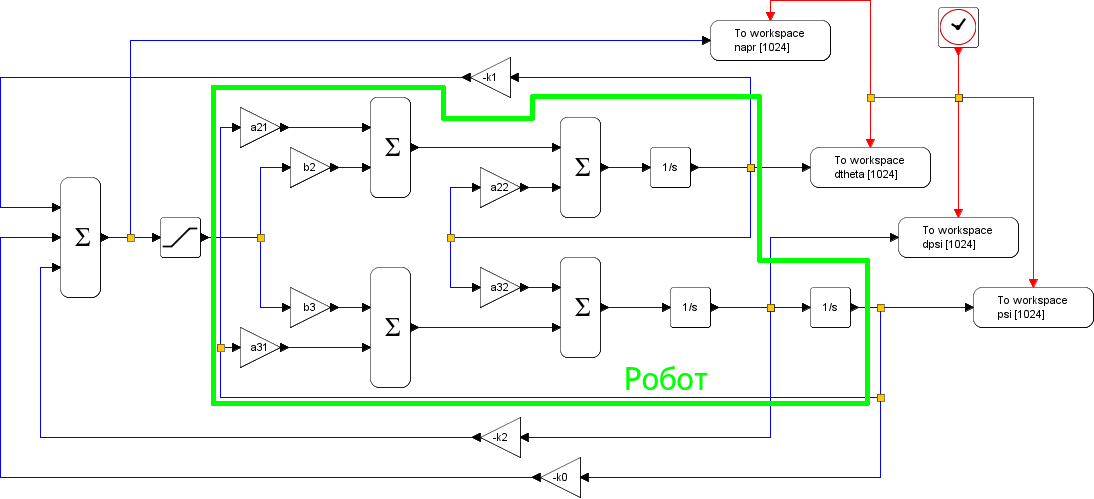
\includegraphics[scale=0.61]{struct_sheme.png}}
	\caption{Cхема моделирования процесса.}
	\label{struct_sheme}
\end{figure}

Обратите внимание, различные каналы связи соединяются только в местах, помеченных оранжевыми квадратиками.
Величины k0, k1 и k2 есть соответствующие элементы матрицы~$K$.
Входящий в эту схему блок с рисунком ломаной, нужен ровно для того же, для чего он использовался в схеме из лабораторной~№3: он ограничивает поступающее на свой вход напряжение определенными границами $-U_{max}$ и $U_{max}$. 

\newpage
\section{Цель работы}
Познакомиться с различными способами расчета коэффициентов \textit{П-регулятора состояния}\lefteqn.\footnote{Так называется применяемая управляющая стратегия.}
Доделать робототехнический механизм, написав для него управляющую программу.

\section{Порядок выполнения работы}
\begin{enumerate}
	\item Используя по крайней мере один из описанных в пособии методов, рассчитайте коэффициенты регулятора.
	Учтите, что получающиеся в ходе расчетов коэффициенты в зависимости от своего физического смысла измеряются или в $\text{В}/\text{рад}$, или в $\text{В}\cdot\text{с}/\text{рад}$.
	\item Напишите для робота в среде BricxCC управляющую программу.
	В~ее основе должен лежать П-регулятор состояния, а следовательно должны использоваться найденные ранее коэффициенты.
	\item Загрузите программу в командный блок и проверьте работоспособность робота.
	В~случае отрицательного результата измените время переходного процесса $t_n$ и повторите расчет со всеми последующими действиями.
	В~случае повторных неудач, продолжайте изменять время переходного процесса и заново проделывать все необходимые действия.
	\item Постройте в Xcos схему моделирования разрабатываемого робота.
	Для нескольких наборов начальных условий~--- значений переменных dpsi0, dtheta0, psi0~--- промоделируйте исследуемый процесс и постройте соответствующие графики.
\end{enumerate}

\end{document}

